\documentclass[10pt,a4paper]{article}
\usepackage[latin1]{inputenc}
\usepackage[spanish]{babel}
\usepackage{amsmath}
\usepackage{amsfonts}
\usepackage{amssymb}
\usepackage{graphicx}
\author{Santiago Videla - Francisco Javier Herrero}
\title{Pr\'actico Especial I: Simulaci\'on Mediante Eventos Discretos}
\pagestyle{headings}
\begin{document}
\maketitle
\newpage
\tableofcontents
\newpage
\section{Introducci\'on}
El enfoque propuesto para realizar la simulaci\'on consiste en la abstracci\'on
del concepto de eventos con el fin de unificar su tratamiento y conseguir asi,
una implementaci\'on mas simple y compacta.

El sistema mantiene actualizada una \textit{unica} lista de eventos por ocurrir. 
Esta lista de eventos garantiza que cada evento se agrega a la lista de manera
ordenada por los tiempos de ocurrencia y que cuando un evento se extrae de
la lista, dicho evento es el mas pr\'oximo a ocurrir. Al extraerse el pr\'oximo evento, 
los subsiguientes eventos en la lista disminuyen su tiempo de ocurrencia, de manera
que representen el tiempo desde la ocurrencia extra\'ida hasta la pr\'oxima.  

A su vez se implement\'o una abstracci\'on del lavadero, con una lista de eventos,  
tiempo principal del sistema, los par\'ametros $N$ (lavarropas), $O$ (operarios) y 
$S$ (repuestos) y los tiempos medios de fallo y reparaci\'on. 
Los detalles del algoritmo pueden observarse en los comentarios de la fuente.

\section{Resultados de las simulaciones}

\begin{table}[ht]
\caption{5 lavarropas, 2 repuestos, 1 operario}
\centering
\begin{tabular}{c c c}
\hline\hline
Iteraciones & Promedio(meses) & Desviaci\'on Estandar(meses) \\ [0.5ex]
\hline
1 & 2.008329 & 0.000000 \\
10  & 2.187058 & 2.169712 \\
100 & 1.882441 & 1.622037 \\
1000 & 1.717552 & 1.667455 \\
10000 & 1.761247 & 1.624259 \\
\hline
\end{tabular}
\end{table}

\begin{table}[ht]
\caption{5 lavarropas, 3 repuestos, 1 operario}
\centering
\begin{tabular}{c c c}
\hline\hline
Iteraciones & Promedio(meses) & Desviaci\'on Estandar(meses) \\ [0.5ex]
\hline
1 & 3.816586 & 0.000000\\
10 & 3.072992 & 1.610918\\
100 & 3.689234 & 3.551355\\
1000 & 3.429950 & 3.160441\\
10000 & 3.601015 & 3.381243\\
\hline
\end{tabular}
\end{table}

\begin{table}[ht]
\caption{5 lavarropas, 2 repuestos, 2 operarios}
\centering
\begin{tabular}{c c c}
\hline\hline
Iteraciones & Promedio(meses) & Desviaci\'on Estandar(meses) \\ [0.5ex]
\hline
1 & 4.127406 & 0.000000\\
10 & 2.370329 & 1.860703\\
100 & 2.841226 & 2.991606\\
1000 & 2.555216 & 2.388780\\
10000 & 2.561495 & 2.436244\\
\hline
\end{tabular}
\end{table}

\begin{figure}
  \centering
  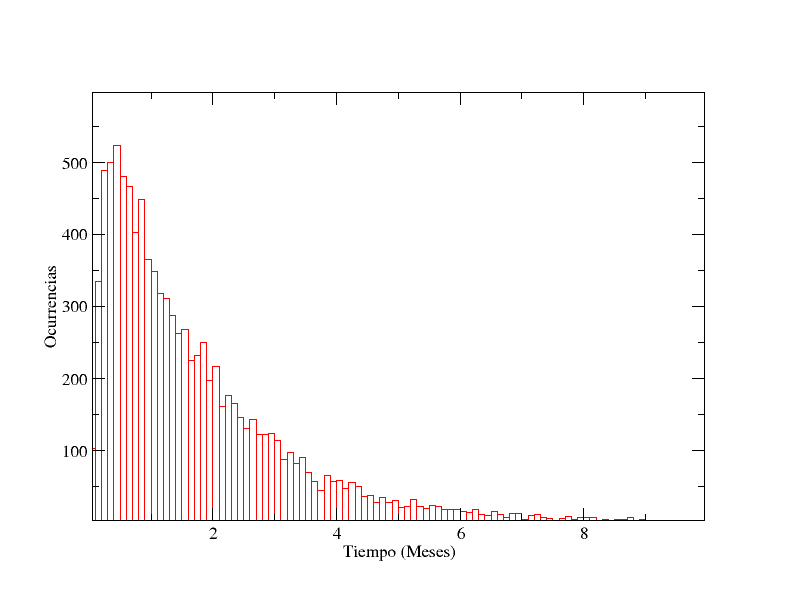
\includegraphics[scale=0.45]{5-2-1.png} 
  \caption{5 lavarropas, 2 repuestos, 1 operario}
  \label{sim:1}
\end{figure}

\begin{figure}
  \centering
  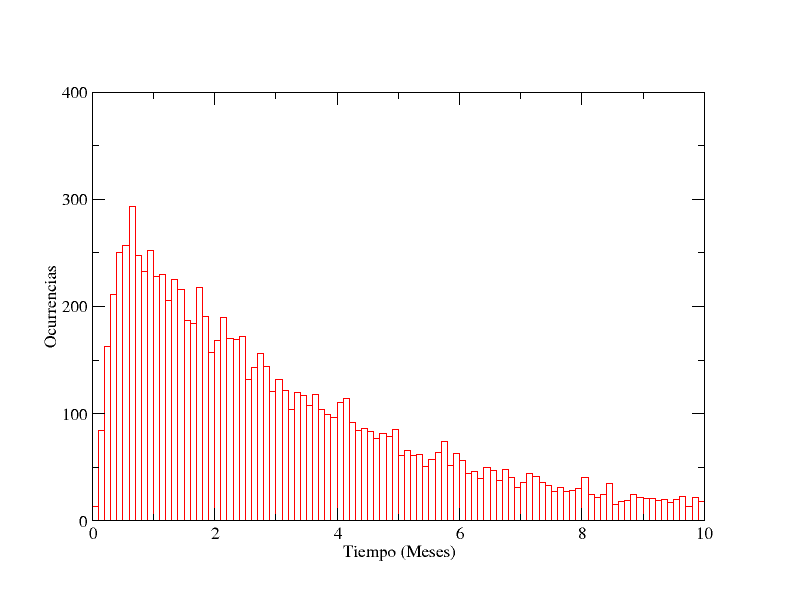
\includegraphics[scale=0.45]{5-3-1.png} 
  \caption{5 lavarropas, 3 repuestos, 1 operario}
  \label{sim:2}
\end{figure}

\begin{figure}
  \centering
  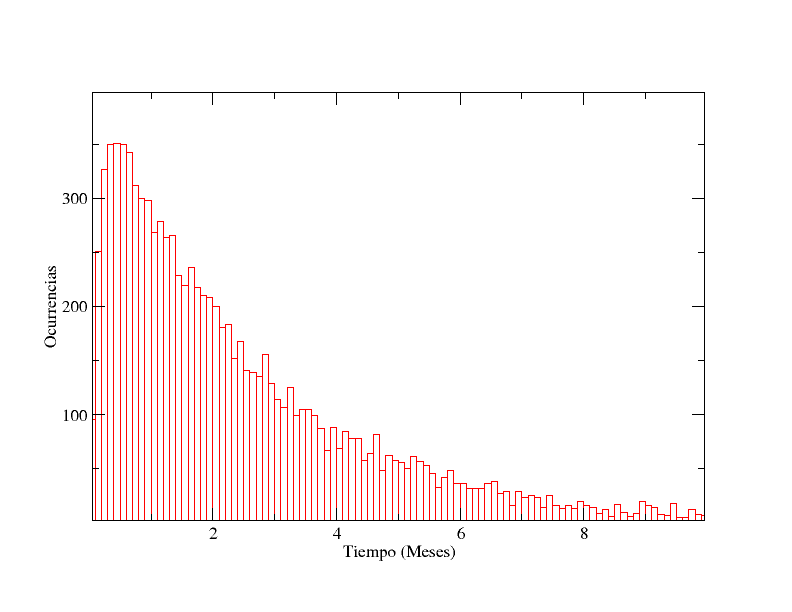
\includegraphics[scale=0.45]{5-2-2.png} 
  \caption{5 lavarropas, 2 repuestos, 2 operarios}
  \label{sim:3}
\end{figure}


\section{Conclusiones}
Observamos por un lado que tanto agregar una maquina de repuesto
como agregar un operario, mejoran significativamente el tiempo medio
que transcurre hasta que el lavadero deja de ser operativo.

Pero entre estas dos mejoras, se puede ver que el hecho de agregar
una maquina de repuesto, conduce a mejores resultados en promedio.
Esto de desprende claramente de los resultados obtenidos en cada una
de las simulaciones como as\'i tambi\'en, de la observaci\'on de los histogramas 
realizados para cada caso.

Observando los histogramas, se puede ver que agregar un operario
(figura~\ref{sim:3}) mejora el tiempo promedio, pero mantiene un numero alto de
fallas para tiempos entre 0 y 1. En cambio, al agregar una maquina de
repuesto (figura~\ref{sim:2}), vemos que el numero de fallas entre 0 y 1, bajan
considerablemente.

\end{document}
